\documentclass[11pt]{article}

\usepackage[margin=1in]{geometry}
\usepackage{times}
\usepackage{graphicx}
\usepackage{booktabs}
\usepackage{multirow}
\usepackage{amsmath}
\usepackage{url}
\usepackage[numbers,sort&compress]{natbib}

\title{MemUpdateBench: Diagnosing Stale Same-Slot Contamination in External Memory}
\author{Anonymous Authors}
\date{}

\begin{document}
\maketitle

\begin{abstract}
External memory systems let language-model agents persist facts across sessions, but repeated updates create a distinct answer-time risk: obsolete values can remain in memory and contaminate the context even when the final value is still recoverable. We study this stale same-slot contamination with MemUpdateBench, a controlled diagnostic benchmark where the same \((\mathrm{entity}, \mathrm{attribute})\) slot is updated across increasing frequencies while same-name distractors and semantic near-miss NOOP events test grounding and parsing robustness. The benchmark separates four quantities that are often conflated: final-state reliability, stale same-slot burden, memory compactness, and slot-conditioned answer robustness.

On the P6.3 hard update-frequency suite, append-only and heuristic memory managers preserve final-state recoverability under oracle slot-state evaluation, reaching state accuracy 1.00 even at \(k=16\). However, they retain stale same-slot entries and collapse under slot-conditioned answering: raw append reaches only 0.07 / 0.10 EM/F1 at \(k=16\) with 14.25 stale same-slot entries. A slot-aware latest-per-slot retrieval rewrite raises raw-add \(k=16\) dev EM from 0.14 to 0.69. Across Qwen, Llama, and Mistral, this stale filtering recovers each model to approximately its own zero-stale slot-prompt ceiling: Qwen 0.69 vs. 0.70, Llama 0.29 vs. 0.27, and Mistral 0.72 vs. 0.72. Controlled mechanism probes further show that stale collapse depends on value conflict, context order, version ambiguity, and repetition or formatting dilution rather than a single majority-vote effect. These results show that stale same-slot context is the dominant stale-specific answer-layer obstacle, while residual errors reflect retrieval, distractor selection, and model-specific clean-context answering limits.
\end{abstract}

\section{Introduction}

External memory gives language-model agents a way to carry user preferences, facts, and task state across long interactions. Most evaluation settings ask whether a system can retrieve a relevant fact after it has been written. In realistic use, however, memory is not only accumulated; it is repeatedly revised. A user may move cities multiple times, change a preferred name, update a project deadline, or correct an earlier statement. These cases stress the same memory slot repeatedly, and the central question becomes not simply whether the final value is present, but whether obsolete values remain and interfere with later answers.

MemUpdateBench focuses on this repeated same-slot update regime. The benchmark isolates updates of the form \((\mathrm{entity}, \mathrm{attribute}) \rightarrow \mathrm{value}\), with actions represented as \texttt{ADD}, \texttt{UPDATE}, and \texttt{NOOP}. This exact slot structure lets us diagnose failure modes that broad memory-agent benchmarks often merge together: stale value retention, missed final updates, wrong entity grounding, wrong attribute parsing, and answer-layer failures. We treat update frequency \(k\) as the main independent variable because it directly controls how many stale same-slot values a non-compacting memory system can accumulate.

This diagnostic setup reveals an important gap between oracle-like memory-state evaluation and answer robustness. Under exact slot lookup, append-only memory can still expose the final value even when many obsolete values remain in the memory bank. Under slot-conditioned answering, the answer layer must condition on the memory contents as a whole, and stale same-slot entries can dominate or confuse generation. The result is a tradeoff among final-state reliability, stale burden, memory compactness, and answer robustness.

Our contribution is a controlled benchmark and analysis package for this update regime. We provide update-frequency splits, deterministic slot-based diagnostics, cluster-backed verification of the main \(k=16\) anchors, mechanism probes for stale context collapse, a three-model ceiling-recovery analysis, and a reproducible workflow for analyzing how memory managers move along the reliability--compactness--robustness curve. MemUpdateBench is complementary to broader long-term memory and agent-memory evaluations such as LoCoMo, LongMemEval, AMemGym, Ledger-QA/UMA, and related persistent-memory settings \citep{locomo,longmemeval,amemgym,ledgerqa_uma}. It is narrower by design: it isolates repeated revisions to a single inspectable slot.

\section{Benchmark}

MemUpdateBench represents memory updates with three actions:
\begin{center}
\begin{tabular}{l}
\texttt{ADD <entity>.<attribute> = <value>} \\
\texttt{UPDATE <entity>.<attribute> = <value>} \\
\texttt{NOOP}
\end{tabular}
\end{center}

The central invariant is exact slot resolution by \((\mathrm{entity}, \mathrm{attribute})\). Each example defines a target slot, a final gold value, distractor entities or attributes, and events that should either update the slot, add other facts, or be ignored as NOOPs. This structure lets the benchmark distinguish state-management failures from answer-generation failures.

The main P6.3 hard split varies update frequency with \(k \in \{1,2,4,8,16\}\). Larger \(k\) means more repeated updates to the same target slot. This controlled axis stresses whether a memory system overwrites stale values, appends new evidence without compacting old evidence, or loses track of the final value. The hard split also includes same-name multi-entity distractors and semantic near-miss NOOP events so that success requires resolving the intended entity and attribute rather than reacting to surface lexical overlap.

The benchmark is intentionally narrow. It does not attempt to cover every memory-agent behavior; instead, it makes one failure pressure measurable. Because each example has an exact target slot and final gold value, we can compute both whether the final state is recoverable and how many obsolete same-slot values remain in memory.

\section{Methods and Evaluation}

We report two complementary answer modes. \texttt{slot\_direct} is oracle-like slot-state evaluation: it checks whether the final value can be resolved for the target \((\mathrm{entity}, \mathrm{attribute})\) slot. \texttt{slot\_prompt} is slot-conditioned answering: it asks the model to answer under a slot-conditioned prompt using the memory contents. The gap between these modes is central to the paper.

We report four metrics together: state accuracy under \texttt{slot\_direct}, EM/F1 under \texttt{slot\_prompt}, stale same-slot entry count, and final memory size. State accuracy measures final-state reliability, EM/F1 measures answer robustness, stale count measures obsolete same-slot burden, and final memory size measures compactness.

The main comparison includes Constrained CRUD, Raw append, Heuristic CRUD, and Long25. Constrained CRUD is an oracle-like diagnostic upper bound: it performs exact slot updates and removes stale same-slot values by construction, so it should not be read as a deployable external-memory framework. Raw append is an append-only baseline that keeps all observed evidence, making stale burden visible. Heuristic CRUD is a partial-compaction baseline with rule-based update behavior. Long25 is a learned compact manager checkpoint from the constrained-slot curriculum; it is included as a compactness/reliability tradeoff point rather than as a final repaired method.

No single metric is sufficient for this setting. State accuracy alone can hide stale evidence, memory size alone can reward overly aggressive deletion, and EM/F1 alone can conflate state-management and answer-layer failures. The paper therefore reports all four metrics together.

\section{Main Results}

\begin{figure}[t]
  \centering
  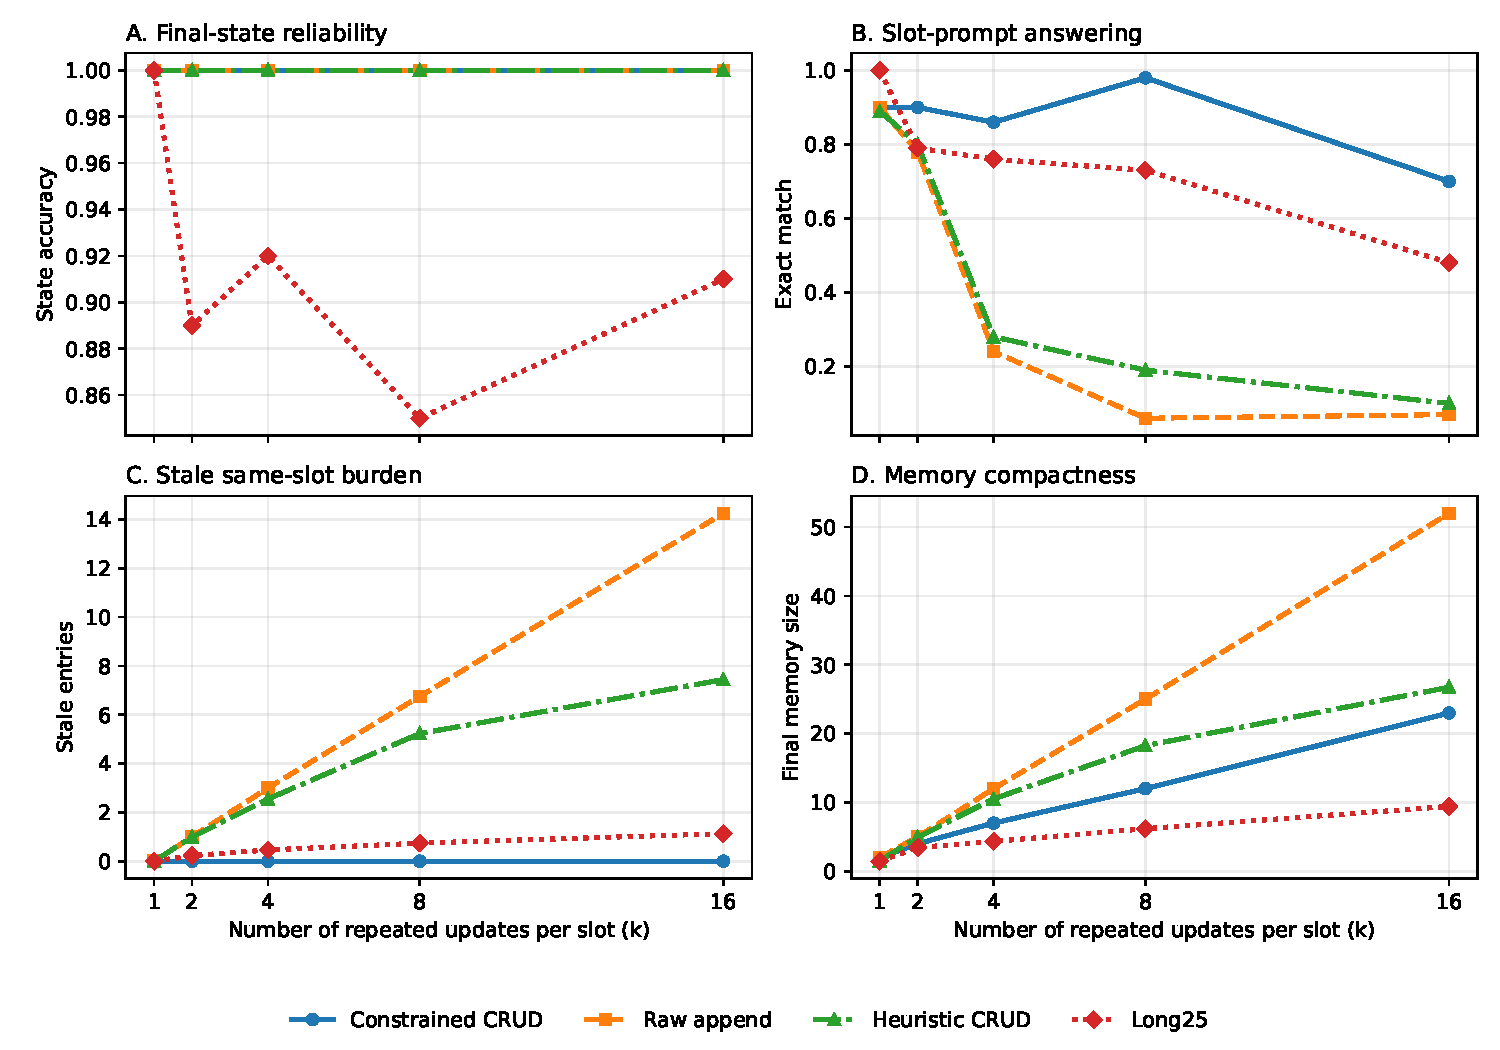
\includegraphics[width=0.88\linewidth]{p63_update_frequency_tradeoff.pdf}
  \caption{Update-frequency stress test on P6.3 hard splits. Oracle-like slot-direct state evaluation hides stale-memory burden for append-only and heuristic methods, while slot-prompt answering reveals answer collapse as repeated same-slot updates accumulate stale entries. Long25 is substantially more compact but sacrifices final-state reliability under hard distractors.}
  \label{fig:p63-update-frequency-tradeoff}
\end{figure}

Figure~\ref{fig:p63-update-frequency-tradeoff} summarizes the update-frequency stress test. Under oracle-like slot-state evaluation, Constrained CRUD, Raw append, and Heuristic CRUD all maintain state accuracy 1.00 through \(k=16\): the final value remains recoverable even after many repeated updates. Under slot-conditioned answering, however, append-style memory collapses. Raw append falls from 0.90 / 0.91 EM/F1 at \(k=1\) to 0.07 / 0.10 at \(k=16\) on the hard test split, and the \(k=16\) dev diagnostic shows the same failure at 0.14 / 0.17 under normal top-\(k\) retrieval. At this endpoint Raw append retains 14.25 stale same-slot entries and final memory size 52.00. Thus the problem is not whether the final value exists somewhere in memory, but whether obsolete same-slot entries contaminate the answer context.

\begin{table}[t]
\centering
\small
\begin{tabular}{lrrrr}
\toprule
Method & State acc. & EM/F1 & Stale & Memory size \\
\midrule
Constrained CRUD & 1.00 & 0.70 / 0.70 & 0.00 & 23.00 \\
Raw append & 1.00 & 0.07 / 0.10 & 14.25 & 52.00 \\
Heuristic CRUD & 1.00 & 0.10 / 0.13 & 7.44 & 26.73 \\
Long25 & 0.91 & 0.48 / 0.53 & 1.13 & 9.43 \\
\bottomrule
\end{tabular}
\caption{High-frequency \(k=16\) tradeoff among final-state reliability, slot-prompt answer quality, stale same-slot burden, and memory compactness. Append-only and heuristic managers preserve slot-direct recoverability but collapse under slot-prompt answering; Long25 is compact but not fully reliable.}
\label{tab:p63-k16-tradeoff}
\end{table}

A retrieval-time intervention isolates the stale-specific component of this collapse. Keeping raw-add writes unchanged but retrieving from the full store and exposing only the latest entry per slot raises \(k=16\) dev EM/F1 from 0.14 / 0.17 to 0.69 / 0.70 while leaving the stored memory unchanged. The same intervention remains strong across update frequencies and on the expanded split, where \(k=16\) reaches 0.750 / 0.764 with stale retrieved rate 0.000. Because this changes answer-time retrieval scope, we treat it as a diagnostic stale-filtering intervention rather than a proposed deployable memory manager.

The high-frequency endpoint also shows why MemUpdateBench reports multiple axes. Constrained CRUD has zero stale same-slot entries and state accuracy 1.00, but still obtains only 0.70 / 0.70 under slot-prompt answering, exposing a clean-memory answer-layer ceiling. Long25 occupies a different tradeoff point: it is much more compact and has lower stale burden than Raw append, but its original \(k=16\) checkpoint has imperfect final-state reliability. These results are not a single method ranking. They show that final-state reliability, stale burden, memory compactness, and answer robustness must be reported separately.

\begin{table}[t]
\centering
\small
\begin{tabular}{lrrrr}
\toprule
Model & Normal raw add & Latest-per-slot & Zero-stale ceiling & Gap \\
\midrule
Qwen2.5-7B & 0.110 & 0.690 & 0.700 & -0.010 \\
Llama3.1-8B & 0.060 & 0.290 & 0.270 & +0.020 \\
Mistral-7B & 0.080 & 0.720 & 0.720 & 0.000 \\
\bottomrule
\end{tabular}
\caption{Ceiling recovery across answer models on P6.3 hard \(k=16\) dev. Normal raw-add retrieval collapses for all three models under stale-contaminated top-\(k\) contexts. Latest-per-slot filtering removes stale retrieved entries and recovers each model to approximately its own zero-stale constrained CRUD slot-prompt ceiling. Absolute EM levels differ mostly because models have different clean-context slot-prompt ceilings.}
\label{tab:ceiling-recovery}
\end{table}

The central multi-model result is ceiling recovery. On \(k=16\) dev, stale-contaminated normal retrieval collapses across Qwen, Llama, and Mistral. After latest-per-slot filtering, each model recovers to approximately its own zero-stale constrained CRUD slot-prompt ceiling: Qwen 0.690 vs. 0.700, Llama 0.290 vs. 0.270, and Mistral 0.720 vs. 0.720. The absolute EM levels differ, but the stale-specific loss is largely removed in each case. This suggests that stale same-slot contamination is the dominant answer-layer obstacle introduced by append-style repeated updates, while remaining differences reflect model-specific clean-context and instruction-following ceilings.

\section{Mechanism and Error Analysis}

The latest-per-slot intervention shows that stale same-slot exposure is a major causal driver, but it does not by itself explain why answer generation collapses. P8.0 therefore adds controlled context-presentation and synthetic same-slot probes. In real raw-add \(k=16\) dev contexts, holding retrieved entries fixed while changing only presentation changes EM substantially: normal order gives EM/F1 0.110 / 0.136, chronological order improves to 0.230 / 0.275, reverse chronological falls to 0.010 / 0.050, timestamp annotation reaches 0.150 / 0.200, and explicit \texttt{[latest]} / \texttt{[outdated]} labels reach 0.260 / 0.298. Because gold retrieval, stale retrieval rate, and retrieved stale count are identical across these conditions, the differences reflect answer-layer context use rather than retrieval composition.

\begin{table}[t]
\centering
\small
\begin{tabular}{lrrrrr}
\toprule
Condition & EM & F1 & Ans. val. & Gold ret. & Stale avg. \\
\midrule
Normal order & 0.110 & 0.136 & 0.140 & 0.360 & 4.040 \\
Chronological & 0.230 & 0.275 & 0.320 & 0.360 & 4.040 \\
Reverse chronological & 0.010 & 0.050 & 0.010 & 0.360 & 4.040 \\
Timestamp labels & 0.150 & 0.200 & 0.230 & 0.360 & 4.040 \\
Latest/outdated labels & 0.260 & 0.298 & 0.350 & 0.360 & 4.040 \\
Current first & 0.020 & 0.060 & 0.020 & 0.360 & 4.040 \\
Current last & 0.040 & 0.080 & 0.040 & 0.360 & 4.040 \\
\bottomrule
\end{tabular}
\caption{Real-context mechanism probe on raw append \(k=16\) dev. Retrieved composition is fixed across rows: gold retrieval is 0.360 and retrieved stale count is 4.040. Changes in EM therefore reflect answer-layer sensitivity to context presentation rather than retrieval composition.}
\label{tab:real-context-mechanism}
\end{table}

A synthetic same-slot probe isolates gold-present behavior more cleanly. With conflicting stale values and no labels, reverse chronological contexts collapse immediately: one stale entry after the current value yields EM 0.188, and two or more stale entries are near zero. Explicit latest/outdated labels almost completely repair this conflict-driven collapse. Chronological conflict contexts are much more robust, reaching EM 0.750 even at stale=16, which rules out a simple majority-vote-only story. When stale entries repeat the current value, answer-value-present remains 1.000 but exact EM drops at higher repetition, indicating a separate repetition or formatting-dilution effect. A stricter Lost-in-the-Middle-style gold-position probe then fixes the context set and moves only the gold slot entry: Qwen2.5-7B-Instruct reaches EM/F1 0.630 / 0.654 when gold is at the end, but only 0.090 / 0.183 in the middle and 0.010 / 0.073 at the beginning. This directly links stale-context failure to answer-layer position sensitivity and a strong final-position/recency advantage.

\begin{figure}[t]
  \centering
  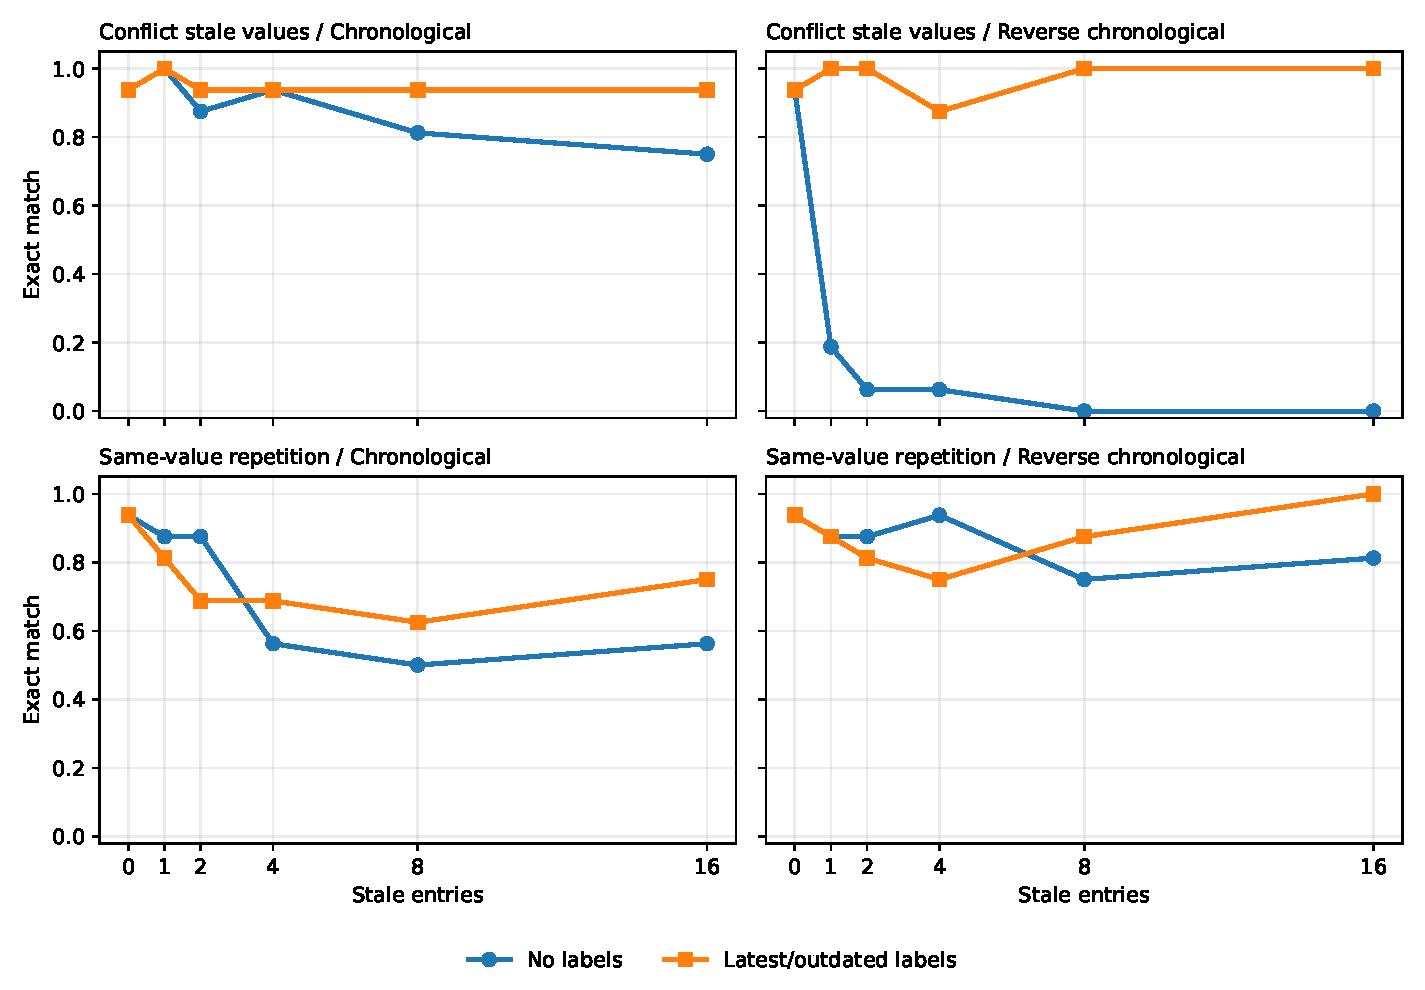
\includegraphics[width=0.88\linewidth]{figures/p80_synthetic_same_slot_matrix.pdf}
  \caption{Synthetic same-slot probes isolate gold-present answer behavior by controlling stale count, value conflict, order, and explicit version labels. Conflict plus reverse chronological order collapses without labels, while latest/outdated labels largely repair the failure. Same-value repetition still reduces exact EM at high stale counts despite answer-value-present staying 1.000.}
  \label{fig:synthetic-same-slot}
\end{figure}

\begin{figure}[t]
  \centering
  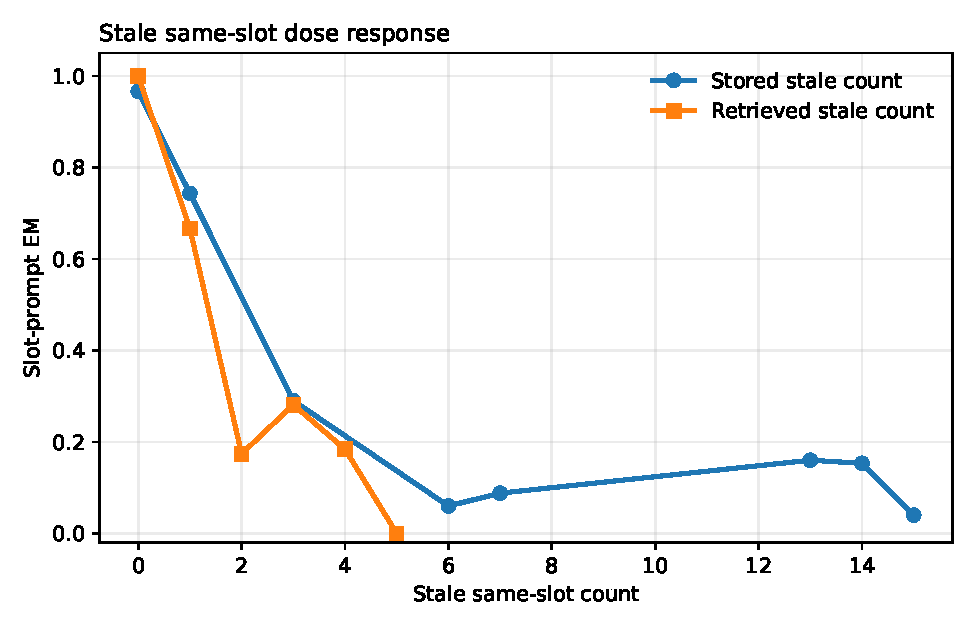
\includegraphics[width=0.88\linewidth]{figures/p80_stale_dose_response.pdf}
  \caption{Dose-response of raw append under slot-conditioned answering. EM falls sharply once stale same-slot entries appear. Retrieved stale exposure has a steeper lightweight logistic slope and lower ED50 than stored stale burden, supporting an answer-context exposure mechanism.}
  \label{fig:stale-dose-response}
\end{figure}

The dose-response analysis reaches the same conclusion from existing benchmark traces. Pooling raw-add slot-prompt runs across P6.3 and expanded all-\(k\) examples, EM drops from 0.967 with zero stored stale entries to 0.743 with one stale entry and 0.290 with three stale entries. A lightweight logistic fit estimates ED50 around 3.18 stored stale entries and 1.89 retrieved stale entries, suggesting that retrieved stale exposure is closer to the answer-time failure mechanism than memory-store pollution alone.

The residual-error analyses separate stale-specific failures from other limits. Constrained CRUD reaches perfect slot-direct state accuracy and zero stale same-slot burden at \(k=16\), yet its slot-prompt EM/F1 remains 0.70 / 0.70, so clean memory state is not sufficient for perfect answer generation. The same pattern appears in the three-model ceiling controls discussed above: once stale same-slot entries are removed, remaining gaps are model-specific clean-context answering limits rather than stale-value selection.

Long25 illustrates the complementary failure mode for compact learned managers. It greatly reduces stale burden and final memory size, but its remaining \(k=16\) state errors are mostly wrong final values under hard distractors rather than wrong entity or wrong attribute grounding. This supports a compactness/reliability interpretation: learned compaction can remove stale evidence, but it must still preserve the latest value exactly.

\section{Discussion}

The central finding is a tradeoff curve, not a simple method ranking. Append-only memory preserves final values under oracle lookup but accumulates stale same-slot evidence that breaks slot-conditioned answering. Heuristic compaction reduces some memory growth but still leaves enough obsolete same-slot evidence to cause severe prompted-answer degradation. Learned compact managers reduce stale burden and memory size, but may miss final updates or remain incompletely compact.

This separation matters for memory-system evaluation. A benchmark that only asks whether the final value is present can miss the practical failure mode where the correct value coexists with many obsolete alternatives. Conversely, a benchmark that only reports answer EM/F1 cannot distinguish whether a failure came from state corruption, stale interference, wrong entity grounding, wrong attribute parsing, or answer-layer behavior. MemUpdateBench is designed to keep these axes separate, so a realistic memory benchmark should report final-state reliability, stale burden, compactness, and answer robustness together.

The current results also motivate, but do not yet perform, method-improvement work. Long25 shows that learning can move a system toward lower stale burden and smaller memory, but its wrong-value failures show that compactness alone is not sufficient. The latest-per-slot retrieval intervention should likewise be read as a mechanism ablation rather than a proposed memory manager: it shows that stale context contamination and failure to surface the latest slot entry explain much of raw append's prompted-answer collapse. The three-model ceiling-recovery result strengthens this interpretation: once stale same-slot entries are removed from the answer context, each model rises to its own clean-memory ceiling, and remaining differences are mainly answer-layer or instruction-following limits rather than unaddressed stale-specific loss. The mechanism probes reinforce that this is a retrieval-and-context story rather than a simple monotonic stale-count story: stale conflict interacts with order and version cues, repeated same-value contexts can still hurt exact answers, and different answer models have different clean-context ceilings. A future repair-training phase should therefore be evaluated against the same four axes rather than optimized only for prompted answer accuracy.

\section{Limitations}

MemUpdateBench is intentionally controlled. The benchmark uses synthetic slot-structured examples rather than unconstrained real user histories, because the goal is to isolate repeated same-slot update behavior and measure stale same-slot burden exactly. This control is also a limitation: real memory systems may face noisier language, implicit updates, uncertain entity boundaries, and facts whose attributes are not explicitly named.

The \texttt{slot\_direct} metric is oracle-like and should not be interpreted as an end-user answering setting. Its role is to separate memory-state reliability from answer-layer robustness. The practical result should be read primarily through \texttt{slot\_prompt}, where stale same-slot entries remain visible to the answer process.

The current main result stops at \(k=16\) because \(k=16\) already separates oracle recoverability from slot-conditioned answer robustness decisively. We do not add \(k=32\) by default; a higher-frequency stress point should be added only if figure design, advisor feedback, or reviewer concerns require a longer tail.

The current comparison does not include a fair external SDK leaderboard row for systems such as Mem0, Letta, MemGPT, or original Memory-R1 \citep{mem0,letta,memgpt,memoryr1}. Instead, we include a transparent extract-then-store diagnostic pipeline with inspectable records: append storage reproduces stale collapse, while slot overwrite removes stale same-slot burden and reaches high slot-prompt EM. This supports diagnostic utility but should not be overclaimed as an ecosystem benchmark. The Mem0 probe shows that a real SDK can be run with inspectable memory state, but the completed off-the-shelf row is only a qualitative dev20 probe. A later text-backend attempt found local Qwen2.5-7B-Instruct and Llama3.1-8B-Instruct weights and fixed the MiniLM embedding device issue, but Mem0's structured extraction parser repeatedly rejected the lightweight server responses before dev3 completed. The repository also contains only a project-local Memory-R1-style approximation, not the original Memory-R1 code/checkpoint.

We also do not start repair training in this paper phase. The present contribution is the benchmark, diagnostic decomposition, and manuscript-ready evidence chain rather than a repaired method result. Long25 should therefore be read as a learned compact manager checkpoint, not as evidence that repair training has solved repeated same-slot updates.

\section{Related Work Positioning}

MemUpdateBench is complementary to broad long-term memory and agent-memory benchmarks such as LoCoMo, LongMemEval, AMemGym, Ledger-QA/UMA, and related multi-session memory evaluations \citep{locomo,longmemeval,amemgym,ledgerqa_uma}. Those settings emphasize realistic memory use across long histories and downstream tasks. MemUpdateBench instead isolates one stressor: repeated revisions to the same \((\mathrm{entity}, \mathrm{attribute})\) slot. This narrow design makes stale same-slot burden directly measurable and separates it from final-state reliability and answer-layer behavior.

External memory systems such as Mem0 and MemGPT/Letta motivate the benchmark because they operationalize persistent memory in agent workflows \citep{mem0,memgpt,letta}. They are important external-validity targets, but they should be included only when the integration exposes enough memory state to compute stale same-slot burden or when the limitation is explicitly reported. Memory editing and dynamic-fact work are also related because repeated updates create conflicts between old and current values, but MemUpdateBench studies inspectable external memory rather than parametric model edits \citep{knowledge_editing_survey}.

The exact slot format also connects to dialogue state tracking, where systems maintain slot-value states across turns \citep{dialogue_state_tracking}. MemUpdateBench borrows this diagnostic clarity while shifting the focus to external memory persistence: the question is not only whether the current state is right, but whether obsolete values remain and later interfere with answers.

\section{Reproducibility}

The source-of-truth chain for the current manuscript is:
\begin{center}
\small
\begin{tabular}{l}
\texttt{results/*/evomemory\_results.json} \\
\(\rightarrow\) \texttt{results/p80\_evidence\_manifest/evidence\_manifest.\{json,csv,md\}} \\
\(\rightarrow\) \texttt{paper/p80\_canonical\_main\_number\_ledger.md} \\
\(\rightarrow\) \texttt{paper/p80\_claim\_evidence\_matrix.md} \\
\(\rightarrow\) \texttt{paper/p80\_paper\_tables.md} and \texttt{paper/figures/p80\_figure\_manifest.json}
\end{tabular}
\end{center}

Canonical regeneration commands, source paths, and claim-to-artifact mappings are documented in the P8 release checklist, canonical number ledger, and claim-evidence matrix. Manuscript-ready tables and figures are collected in the P8 table pack, results-section draft, and figure manifest. The mechanism and replication evidence is documented in the P8 paper notes, including stale dose response, context mechanism probes, synthetic same-slot probes, Lost-in-the-Middle probing, attribute-level error analysis, multi-model stale susceptibility, Mistral third-model replication, and the transparent external extract-then-store diagnostic pipeline.

\bibliographystyle{plainnat}
\bibliography{paper/references_todo}

\end{document}
